
After a bending operation, the sheet is taken to the inspection camera installed on the unloading station.
At this pose, the inspection camera is triggered by the PLC as shown in figure \ref{fig:inspection-setup}. The image is captured and the results are sent to the PLC.

\begin{figure}[h]
    \centering
    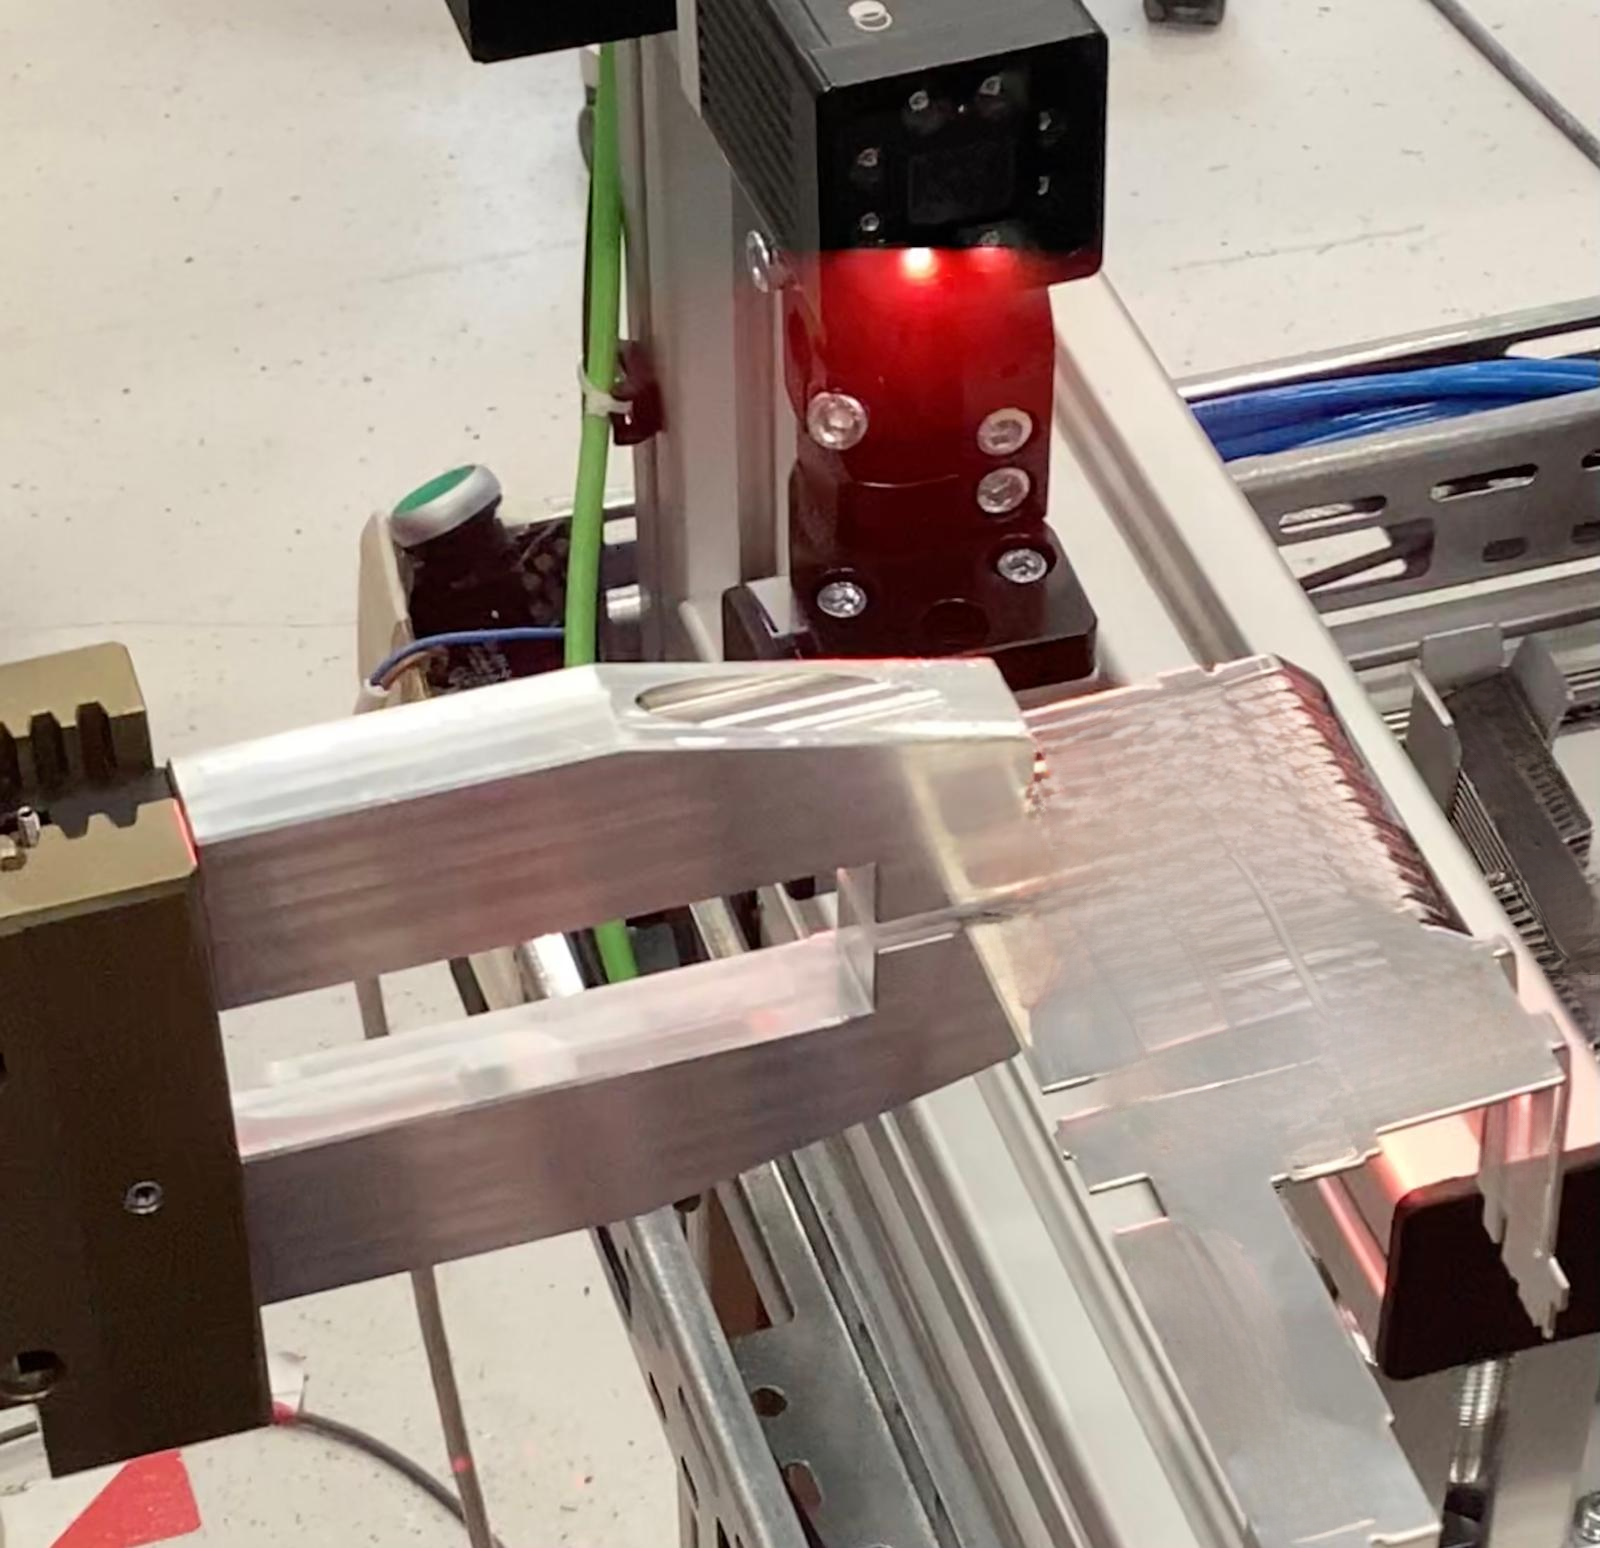
\includegraphics[width=0.6\textwidth]{figures/inspection-setup.png}
    \caption{Robot aligns bent sheet in front of inspection camera}
    \label{fig:inspection-setup}
\end{figure}

The inspection camera measures the bending angle of the sheet metal part. If any discrepancies are detected, the PLC sends feedback to adjust the bending parameters to the bending machine, ensuring continuous improvement in accuracy and quality for the next cycle. These bending parameters are updated by the terminal operating robot.

If the part passes inspection, the KR1410 proceeds to place it in the storage station. If the part fails inspection, it is automatically transferred to a rejection bin under the unloading station.